\documentclass{article}
\usepackage[UTF8]{ctex}
\usepackage{float}
\usepackage{graphicx}

\title{图的模板类设计}
\author{林敬翊}
\date{2022年12月8日}

\begin{document}

\maketitle

\section{邻接表和邻接矩阵}
邻接表(英语:adjacency list)是表示了图中与每一个顶点相邻的边集的集合,这里的集合指的是无序集。\\
~\\
如果是无向图,那么每条边由两个结点组成,分别代表边的两个端点;如果是有向图,那么每条边是一个结点对,分别代表边的始点和终点。\\
~\\
\hspace*{0.7cm}邻接矩阵(英语:adjacency matrix)是一种方阵,用来表示有限图。它的每个元素代表各点之间是否有边相连。\\
~\\
作为特例,简单图的邻接矩阵是(0,1)矩阵并且对角线元素都为0。无向图的邻接矩阵是对称矩阵。图和其邻接矩阵的特征值和特征向量之间的关系是谱图理论的研究对象。\\
~\\
图的关联矩阵需要和邻接矩阵区分。它是图的另一种矩阵表示方式,它的元素表示各个节点-边对是否相关。还有图的度数矩阵,含有每个结点的度数信息。\\
~\\

\section{设计思路}
邻接矩阵采用的是矩阵的存储方式,并且如果是有链接的两个点,将他们双方的矩阵元素都改为1,否则为0.\\

邻接表则是将他们采用vector 和pushback的方式 将他们一一储存在里面。

\section{测试数据与结果}

\begin{figure}[htb]
    \centering
\begin{minipage}[t]{0.48\textwidth}
    \centering
    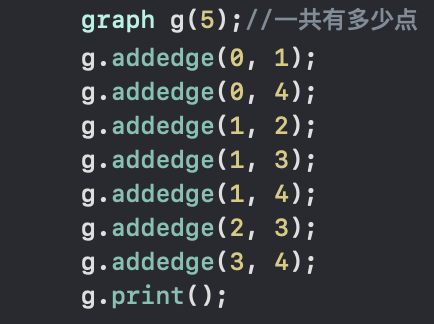
\includegraphics[width=5cm]{data.png}
    \caption{邻接矩阵输入数据}
\end{minipage}
\begin{minipage}[t]{0.48\textwidth}
    \centering
    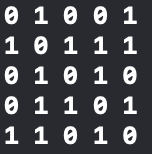
\includegraphics[width=5cm]{conclu.png}
    \caption{邻接矩阵输出结果}
\end{minipage}
\end{figure}

\begin{figure}[htb]
    \centering
\begin{minipage}[t]{0.48\textwidth}
    \centering
    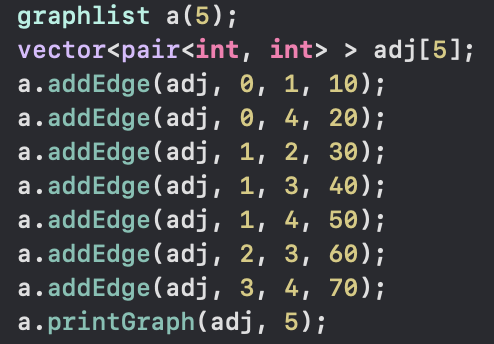
\includegraphics[width=5cm]{data 2.png}
    \caption{邻接表输入数据}
\end{minipage}
\begin{minipage}[t]{0.48\textwidth}
    \centering
    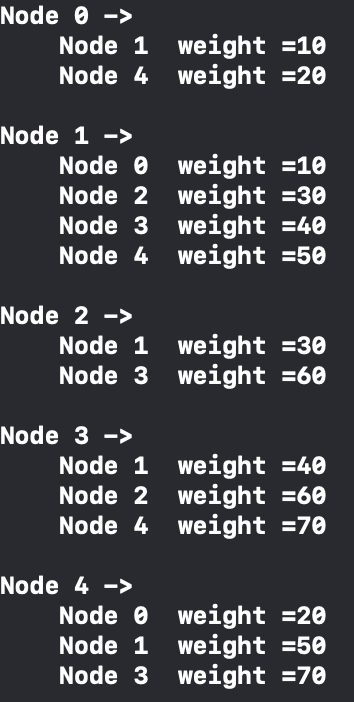
\includegraphics[width=5cm]{conclu 2.png}
    \caption{邻接表输出结果}
\end{minipage}
\end{figure}



\end{document}
